\documentclass[aspectratio=169,10pt]{ctexbeamer}

\usetheme{Madrid}
\usecolortheme{default}
\setbeamertemplate{navigation symbols}{}
\setbeamertemplate{footline}[frame number]

\usepackage{amsmath}
\usepackage{booktabs}
\usepackage{array}
\usepackage{graphicx}
\usepackage{tikz}
\usepackage{xcolor}
\usepackage{listings}
\usetikzlibrary{arrows.meta, positioning}

\definecolor{ucasblue}{RGB}{30,70,120}
\definecolor{ucasgreen}{RGB}{36,120,92}
\definecolor{lightgray}{RGB}{245,247,250}
\definecolor{codeblue}{RGB}{28,68,135}
\definecolor{codegreen}{RGB}{40,120,80}

\setbeamercolor{structure}{fg=ucasblue}
\setbeamercolor{title}{fg=white,bg=ucasblue}
\setbeamercolor{frametitle}{fg=white,bg=ucasblue}
\setbeamercolor{block title}{fg=white,bg=ucasblue}
\setbeamercolor{block body}{bg=lightgray}
\setbeamerfont{frametitle}{series=\bfseries}
\setbeamerfont{title}{series=\bfseries,size=\Large}

\newcolumntype{M}[1]{>{\centering\arraybackslash}m{#1}}
\graphicspath{{../Figure/}}

\lstset{
	language=Python,
	basicstyle=\ttfamily\scriptsize,
	numbers=left,
	numberstyle=\tiny\color{ucasgreen},
	showstringspaces=false,
	breaklines=true,
	frame=single,
	rulecolor=\color{ucasblue!45},
	framerule=0.4pt,
	backgroundcolor=\color{lightgray},
	columns=fullflexible,
	keywordstyle=\bfseries\color{codeblue},
	commentstyle=\itshape\color{codegreen},
	stringstyle=\color{red!65!black},
	tabsize=4
}

\newcommand{\transcard}[4]{
	\fcolorbox{ucasblue!25}{lightgray}{
		\begin{minipage}{0.95\linewidth}
			\textbf{#1}\par\vspace{0.18em}
			\textbf{源句：}#2\par
			\textbf{模型译文：}#3\par
			\textbf{参考译文：}#4
		\end{minipage}
	}
}

\title{实验四：基于Transformer的神经机器翻译}
\subtitle{Chinese-English Neural Machine Translation}
\author{尧祥临 \quad 202518023406038}
\institute{中国科学院大学 \quad 前沿交叉科学学院\\2026年春季学期\quad 深度学习}
\date{}

\begin{document}

\begin{frame}
	\titlepage
\end{frame}

\begin{frame}{实验任务}
	\begin{block}{目标}
		基于 Transformer 实现中英神经机器翻译，完成数据处理、模型训练、测试翻译和 BLEU-4 评估。
	\end{block}

	\begin{columns}[T,onlytextwidth]
		\begin{column}{0.48\textwidth}
			\textbf{实验要求}
			\begin{itemize}
				\item 使用深度学习框架构建机器翻译模型
				\item 实现 Encoder-Decoder 结构
				\item 测试集 BLEU-4 大于 14
			\end{itemize}
		\end{column}
		\begin{column}{0.48\textwidth}
			\textbf{本次结果}
			\begin{itemize}
				\item 训练日志共 57 个 epoch
				\item 最优开发集 loss 出现在第 47 轮
				\item 测试集 BLEU-4：\textbf{14.99}
			\end{itemize}
		\end{column}
	\end{columns}
\end{frame}

\begin{frame}{数据集与预处理}
	\begin{columns}[T,onlytextwidth]
		\begin{column}{0.52\textwidth}
			\begin{itemize}
				\item 数据集：NiuTrans 中英平行语料
				\item 训练集：100000 个句对
				\item 开发集：400 个句对
				\item 测试集：1000 个中文句子
				\item 参考译文：1000 个英文句子
			\end{itemize}
		\end{column}
		\begin{column}{0.44\textwidth}
			\begin{block}{处理方式}
				语料已经分词，代码中直接按空格切分；训练集、开发集和测试集统一编码后保存为 \texttt{processed.pt}。
			\end{block}
			\begin{block}{特殊符号}
				\texttt{<pad>}、\texttt{<bos>}、\texttt{<eos>}、\texttt{<unk>} 用于 padding、序列边界和低频词处理。
			\end{block}
		\end{column}
	\end{columns}
\end{frame}

\begin{frame}{词表与序列编码}
	\begin{columns}[T,onlytextwidth]
		\begin{column}{0.46\textwidth}
			\begin{table}
				\centering
				\small
				\begin{tabular}{l r}
					\toprule
					项目 & 数值 \\
					\midrule
					源语言词表 & 30000 \\
					目标语言词表 & 22811 \\
					最小词频 & 2 \\
					最大序列长度 & 80 \\
					\bottomrule
				\end{tabular}
			\end{table}
		\end{column}
		\begin{column}{0.5\textwidth}
			\begin{block}{编码策略}
				每个源句和目标句都加入 \texttt{<bos>} 与 \texttt{<eos>}，超长句子截断，batch 内使用动态 padding。
			\end{block}
			\begin{block}{为什么缓存}
				词表和 id 序列只需要构造一次，训练和评估复用同一份缓存，避免词表不一致。
			\end{block}
		\end{column}
	\end{columns}
\end{frame}

\begin{frame}{整体流程}
	\centering
	\begin{tikzpicture}[
		node distance=0.45cm,
		flowstep/.style={draw=ucasblue, fill=lightgray, rounded corners=2pt,
			minimum width=2.2cm, minimum height=0.78cm, align=center},
		arrow/.style={-{Latex[length=2mm]}, thick, draw=ucasblue}
	]
		\node[flowstep] (data) {平行语料\\词表构造};
		\node[flowstep, right=of data] (encode) {句子编码\\动态 padding};
		\node[flowstep, right=of encode] (model) {Transformer\\Encoder-Decoder};
		\node[flowstep, right=of model] (train) {Teacher Forcing\\训练};
		\node[flowstep, right=of train] (eval) {贪心解码\\BLEU-4};
		\foreach \a/\b in {data/encode,encode/model,model/train,train/eval}
			\draw[arrow] (\a) -- (\b);
	\end{tikzpicture}

	\vspace{0.75cm}
	\begin{columns}[T,onlytextwidth]
		\begin{column}{0.48\textwidth}
			\textbf{训练阶段}
			\begin{itemize}
				\item 输入中文句子和英文前缀
				\item 预测目标端下一个 token
			\end{itemize}
		\end{column}
		\begin{column}{0.48\textwidth}
			\textbf{测试阶段}
			\begin{itemize}
				\item 只输入中文句子
				\item 从 \texttt{<bos>} 开始逐步生成英文
			\end{itemize}
		\end{column}
	\end{columns}
\end{frame}

\begin{frame}{Transformer 模型结构}
	\centering
	\resizebox{\linewidth}{!}{%
	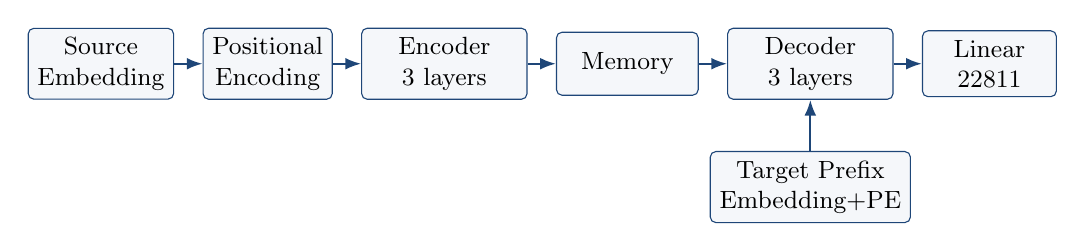
\begin{tikzpicture}[
		layer/.style={draw=ucasblue, fill=lightgray, rounded corners=2pt,
			minimum height=0.8cm, align=center, font=\small},
		arrow/.style={-{Latex[length=2mm]}, thick, draw=ucasblue},
		node distance=0.36cm
	]
		\node[layer, minimum width=1.8cm] (src) {Source\\Embedding};
		\node[layer, minimum width=1.6cm, right=of src] (pe1) {Positional\\Encoding};
		\node[layer, minimum width=2.1cm, right=of pe1] (enc) {Encoder\\3 layers};
		\node[layer, minimum width=1.8cm, right=of enc] (mem) {Memory};
		\node[layer, minimum width=2.1cm, right=of mem] (dec) {Decoder\\3 layers};
		\node[layer, minimum width=1.7cm, right=of dec] (gen) {Linear\\22811};
		\foreach \a/\b in {src/pe1,pe1/enc,enc/mem,mem/dec,dec/gen}
			\draw[arrow] (\a) -- (\b);
		\node[layer, minimum width=1.8cm, below=0.65cm of dec] (tgt) {Target Prefix\\Embedding+PE};
		\draw[arrow] (tgt) -- (dec);
	\end{tikzpicture}
	}

	\vspace{0.55cm}
	\begin{columns}[T,onlytextwidth]
		\begin{column}{0.48\textwidth}
			\begin{block}{主要配置}
				embedding dim = 256，heads = 8，FFN dim = 512，dropout = 0.1。
			\end{block}
		\end{column}
		\begin{column}{0.48\textwidth}
			\begin{block}{输出方式}
				Decoder 每个位置的隐藏状态经过线性层映射到英文词表，得到 token logits。
			\end{block}
		\end{column}
	\end{columns}
\end{frame}

\begin{frame}[fragile]{前向传播核心代码}
\begin{lstlisting}
def forward(self, src, tgt_input):
    src_key_padding_mask, tgt_key_padding_mask, tgt_mask = create_masks(
        src, tgt_input, self.src_pad_idx, self.tgt_pad_idx
    )

    src_emb = self.positional_encoding(self.src_embedding(src))
    tgt_emb = self.positional_encoding(self.tgt_embedding(tgt_input))

    memory = self.transformer.encoder(
        src_emb,
        src_key_padding_mask=src_key_padding_mask
    )
    output = self.transformer.decoder(
        tgt_emb, memory,
        tgt_mask=tgt_mask,
        tgt_key_padding_mask=tgt_key_padding_mask,
        memory_key_padding_mask=src_key_padding_mask
    )
    return self.generator(output)
\end{lstlisting}
\end{frame}

\begin{frame}{Mask 与训练目标}
	\begin{columns}[T,onlytextwidth]
		\begin{column}{0.48\textwidth}
			\begin{block}{Padding mask}
				忽略 batch 中为了补齐长度加入的 \texttt{<pad>}，避免模型把 padding 当成真实句子内容。
			\end{block}
			\begin{block}{Causal mask}
				Decoder 预测第 $t$ 个 token 时，只能看到 $t$ 之前的目标端前缀，不能提前看到答案后文。
			\end{block}
		\end{column}
		\begin{column}{0.48\textwidth}
			\begin{block}{Teacher forcing}
				\[
					\mathrm{Input}=y_0,\ldots,y_{T-2}
				\]
				\[
					\mathrm{Target}=y_1,\ldots,y_{T-1}
				\]
			\end{block}
			\begin{itemize}
				\item 损失函数：CrossEntropy
				\item \texttt{ignore\_index} 忽略 padding
				\item label smoothing = 0.1
			\end{itemize}
		\end{column}
	\end{columns}
\end{frame}

\begin{frame}{训练配置}
	\begin{columns}[T,onlytextwidth]
		\begin{column}{0.49\textwidth}
			\begin{table}
				\centering
				\small
				\begin{tabular}{l l}
					\toprule
					项目 & 设置 \\
					\midrule
					Batch size & 64 \\
					Epochs & 60 \\
					Embedding dim & 256 \\
					Encoder layers & 3 \\
					Decoder layers & 3 \\
					Attention heads & 8 \\
					\bottomrule
				\end{tabular}
			\end{table}
		\end{column}
		\begin{column}{0.49\textwidth}
			\begin{table}
				\centering
				\small
				\begin{tabular}{l l}
					\toprule
					项目 & 设置 \\
					\midrule
					Optimizer & AdamW \\
					Learning rate & $5\times10^{-4}$ \\
					Weight decay & $1\times10^{-4}$ \\
					Label smoothing & 0.1 \\
					Scheduler & ReduceLROnPlateau \\
					Gradient clip & 1.0 \\
					\bottomrule
				\end{tabular}
			\end{table}
		\end{column}
	\end{columns}
\end{frame}

\begin{frame}{BLEU-4 指标}
	\begin{columns}[T,onlytextwidth]
		\begin{column}{0.52\textwidth}
			\begin{block}{BLEU 的核心}
				比较模型译文和参考译文之间的 n-gram 重合程度，BLEU-4 同时考虑 1-gram 到 4-gram。
			\end{block}
			\[
				\mathrm{BLEU}=BP\cdot
				\exp\left(\sum_{n=1}^{4}w_n\log p_n\right)
			\]
			\[
				BP =
				\begin{cases}
					1, & c>r,\\
					e^{1-r/c}, & c\le r.
				\end{cases}
			\]
		\end{column}
		\begin{column}{0.43\textwidth}
			\begin{block}{实验结果}
				测试集共有 1000 个句子，当前模型语料级 BLEU-4 为：
				\[
					\mathbf{14.99}
				\]
			\end{block}
			\begin{itemize}
				\item 满足实验要求：BLEU-4 $>14$
				\item 单句 BLEU 波动较大，只作为辅助观察
			\end{itemize}
		\end{column}
	\end{columns}
\end{frame}

\begin{frame}{训练过程}
	\begin{columns}[T,onlytextwidth]
		\begin{column}{0.63\textwidth}
			
\includegraphics[width=\linewidth]{loss_ppl_curves.png}
		\end{column}
		\begin{column}{0.33\textwidth}
			\begin{block}{关键节点}
				\small
				\begin{itemize}
					\item 第 1 轮 dev loss：5.1639
					\item 第 30 轮 dev loss：3.9208
					\item 第 47 轮 dev loss：\textbf{3.8580}
					\item 第 57 轮 dev loss：3.8604
				\end{itemize}
			\end{block}
			\small
			第 47 轮之后训练 loss 仍下降，但开发集 loss 基本不再改善，因此使用开发集最优模型做测试。
		\end{column}
	\end{columns}
\end{frame}

\begin{frame}{学习率与梯度范数}
	\begin{columns}[T,onlytextwidth]
		\begin{column}{0.63\textwidth}
			
\includegraphics[width=\linewidth]{lr_grad_curves.png}
		\end{column}
		\begin{column}{0.33\textwidth}
			\begin{block}{观察}
				\small
				\begin{itemize}
					\item 开发集停滞后降低学习率
					\item 梯度范数整体稳定在 1 附近
					\item 梯度裁剪避免异常更新
				\end{itemize}
			\end{block}
			\small
			这次训练没有出现明显梯度爆炸，后期主要是小幅收敛和轻微过拟合之间的平衡。
		\end{column}
	\end{columns}
\end{frame}

\begin{frame}{译文长度分布}
	\begin{columns}[T,onlytextwidth]
		\begin{column}{0.62\textwidth}
			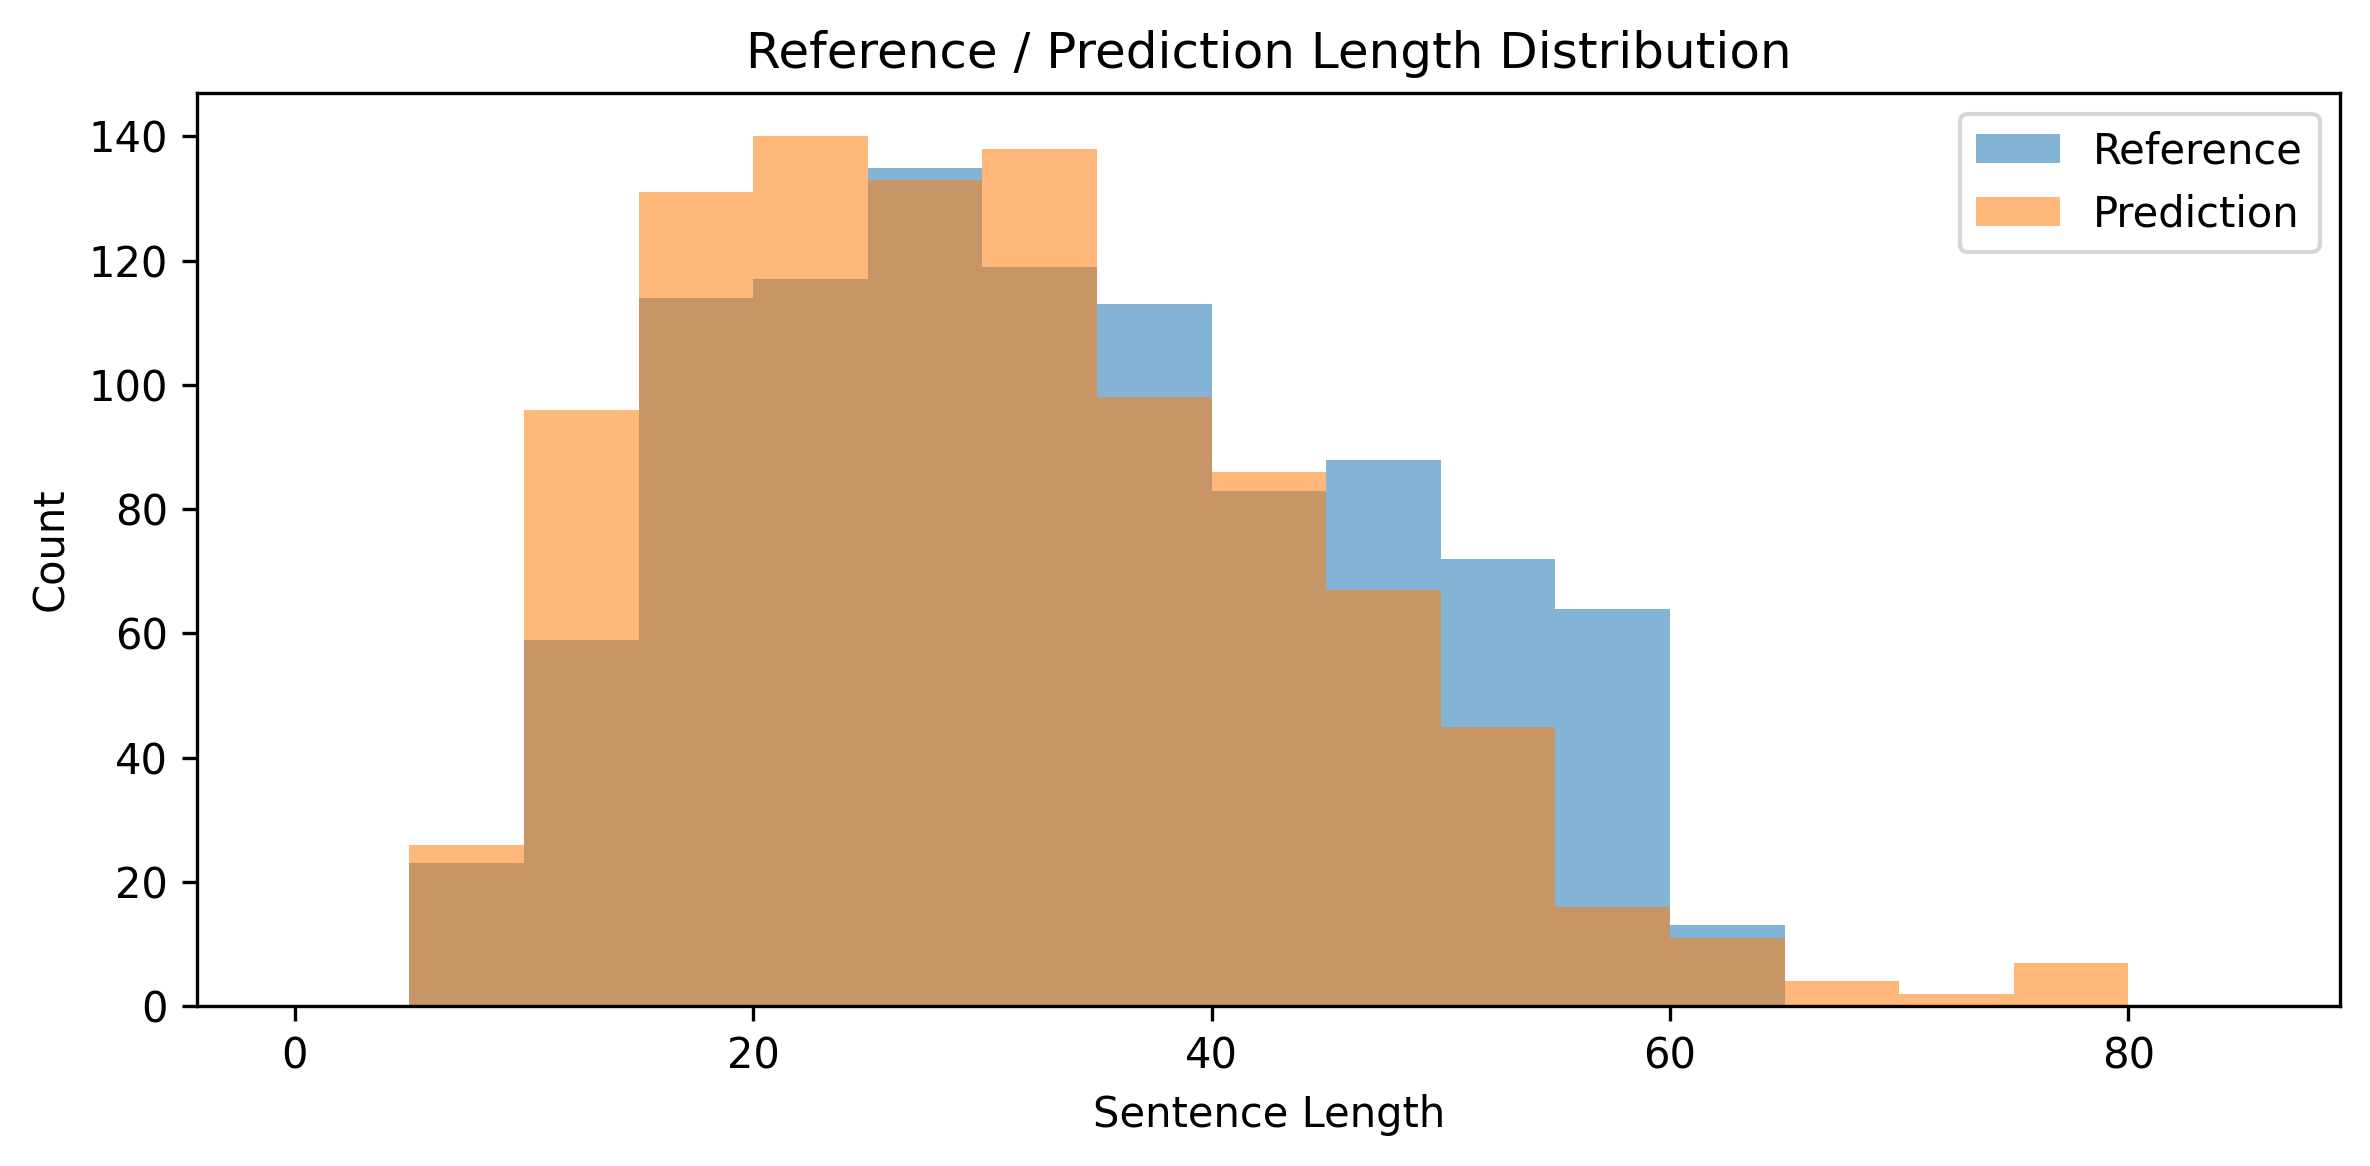
\includegraphics[width=\linewidth]{length_distribution.png}
		\end{column}
		\begin{column}{0.34\textwidth}
			\begin{table}
				\centering
				\small
				\begin{tabular}{l r}
					\toprule
					项目 & 平均长度 \\
					\midrule
					源句 & 24.77 \\
					参考译文 & 32.88 \\
					模型译文 & 29.93 \\
					\bottomrule
				\end{tabular}
			\end{table}
			\small
			模型译文整体接近参考译文，但略短一些，说明模型有时会省略修饰信息或生成偏保守的句子。
		\end{column}
	\end{columns}
\end{frame}

\begin{frame}{单句 BLEU 样例}
	\begin{columns}[T,onlytextwidth]
		\begin{column}{0.57\textwidth}
			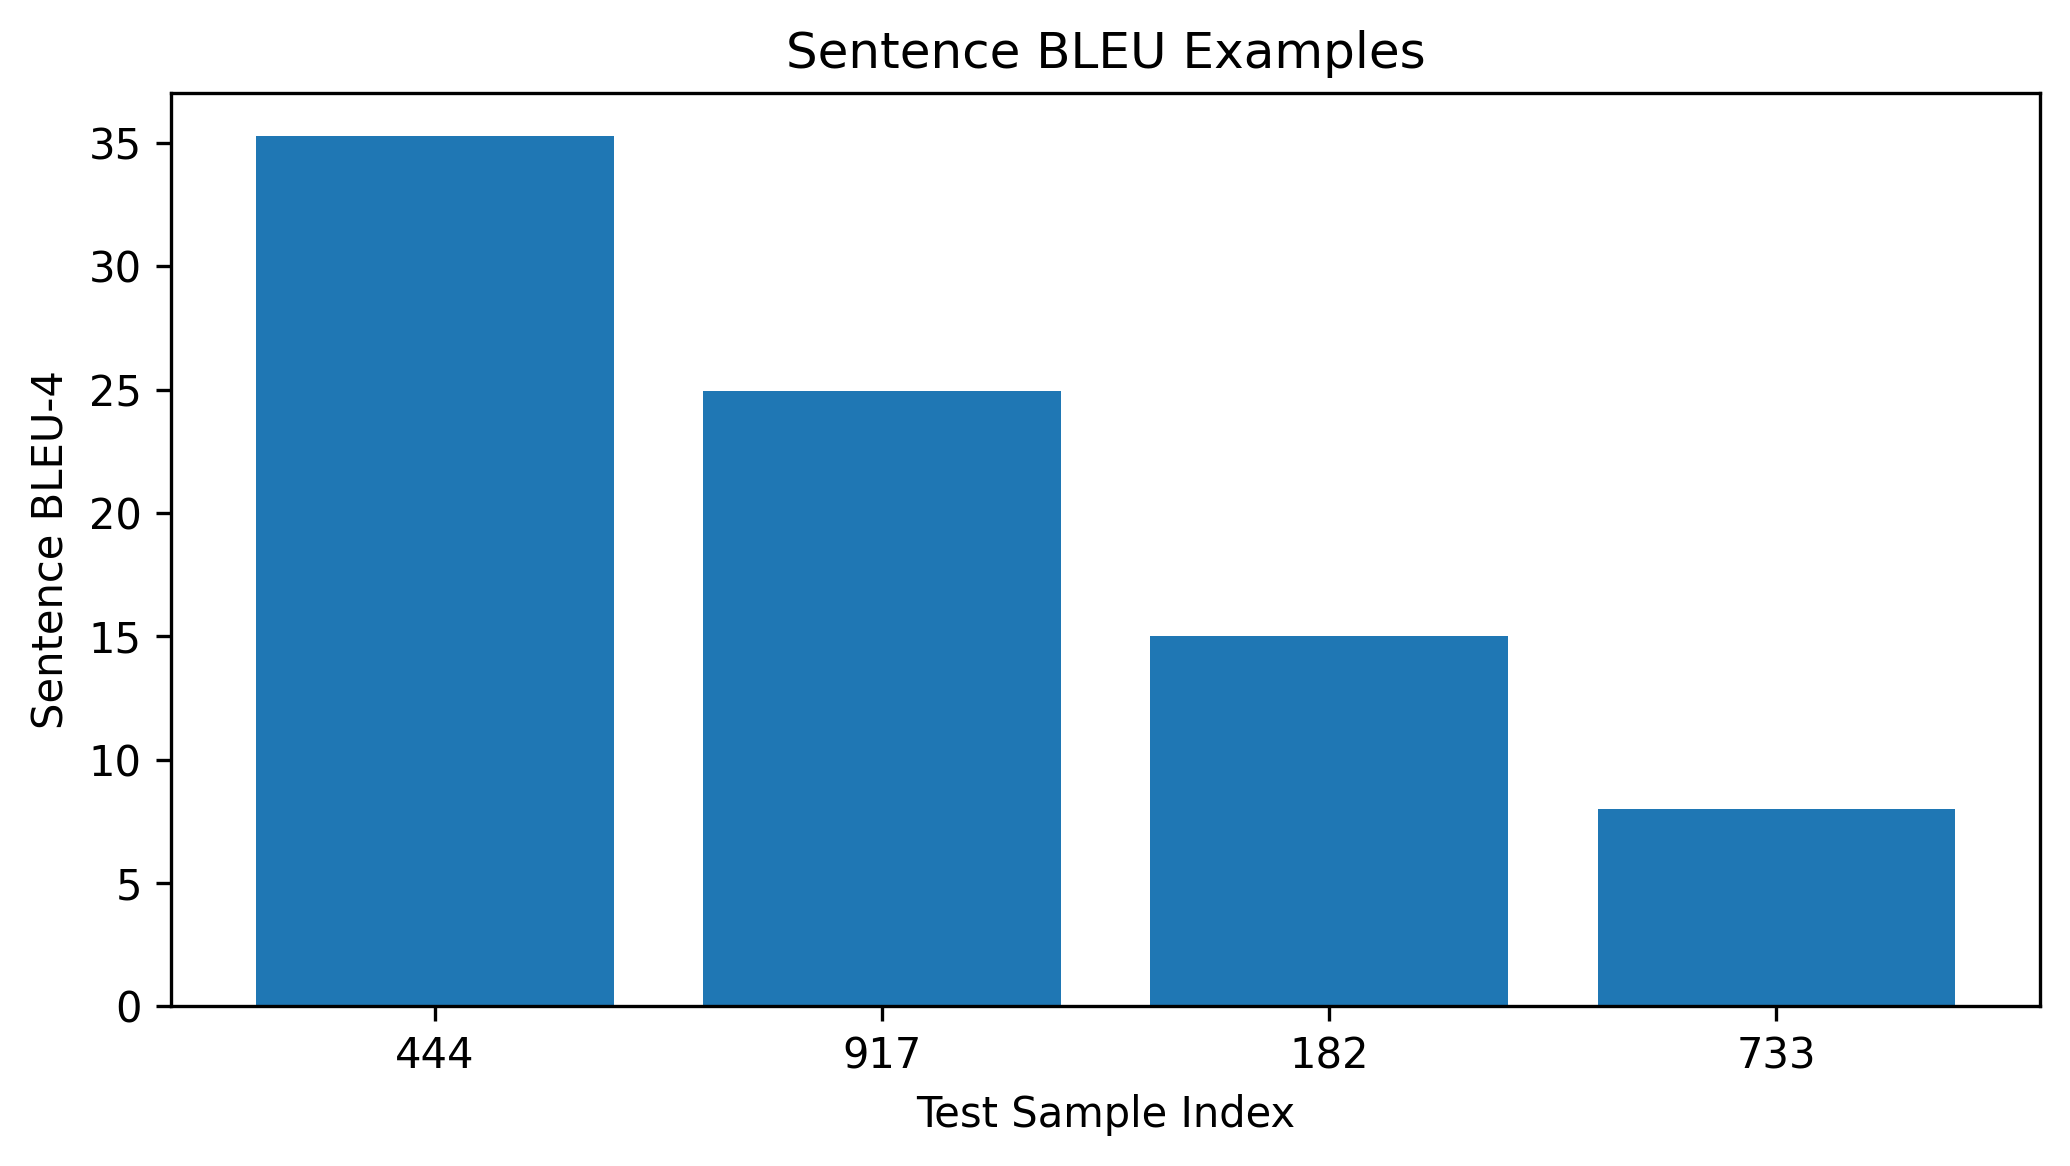
\includegraphics[width=\linewidth]{sentence_bleu_examples.png}
		\end{column}
		\begin{column}{0.39\textwidth}
			\begin{block}{样例观察}
				\small
				\begin{itemize}
					\item 外交文本中的固定表达匹配较好
					\item 多个人名和多重转达关系容易混淆
					\item 数字、低频词和专名会带来 \texttt{<unk>}
					\item 短句上下文少，单句 BLEU 波动更明显
				\end{itemize}
			\end{block}
			\small
			单句 BLEU 不能代替整体 BLEU，但能帮助观察模型到底错在什么地方。
		\end{column}
	\end{columns}
\end{frame}

\begin{frame}{翻译样例：高分句}
	\scriptsize
	\transcard{样例444，BLEU-4=35.27}
	{迟浩田 首先 转达 了 李鹏 委员长 对 布马扎 的 诚挚 问候 和 良好 祝愿 ...}
	{chi haotian first conveyed president jiang zemin 's cordial regards and best wishes to president bouteflika ...}
	{chi haotian first conveyed chairman li peng 's sincere regards and good wishes to boumaza ...}

	\vspace{0.25cm}
	\normalsize
	\begin{block}{模型角度}
		这类外交文本的固定表达比较常见，模型学到了类似 ``conveyed ... regards and best wishes'' 的模板；但句子里人名多、转达关系多，实体关系仍然容易混在一起。
	\end{block}
\end{frame}

\begin{frame}{翻译样例：低分句}
	\scriptsize
	\transcard{样例733，BLEU-4=7.99}
	{若 如此 , 还需要 什 麽 神 盾 舰 ?}
	{if the aegis combat system is so advanced , what kind of aegis combat will be ?}
	{then why do we need aegis ships ?}

	\vspace{0.25cm}
	\normalsize
	\begin{block}{模型角度}
		短句给 Encoder 的上下文较少，模型更依赖训练集中和 ``aegis'' 一起出现的常见搭配；贪心解码每一步选局部最高概率词，容易生成局部常见但整体不贴合源句的短语。
	\end{block}
\end{frame}

\begin{frame}{总结}
	\begin{columns}[T,onlytextwidth]
		\begin{column}{0.48\textwidth}
			\begin{block}{完成内容}
				\begin{itemize}
					\item 完成 NiuTrans 数据处理与缓存
					\item 实现 Transformer Encoder-Decoder
					\item 使用 teacher forcing 训练
					\item 实现贪心解码和 BLEU-4 评估
				\end{itemize}
			\end{block}
		\end{column}
		\begin{column}{0.48\textwidth}
			\begin{block}{结果与不足}
				\begin{itemize}
					\item 测试集 BLEU-4：\textbf{14.99}
					\item 复杂长句仍有实体关系混淆
					\item 词级词表导致低频词和数字不够稳定
					\item 可继续尝试子词分词和 beam search
				\end{itemize}
			\end{block}
		\end{column}
	\end{columns}
\end{frame}

\end{document}
